\chapter{Redes Metabólicas}
 
\indent Neste capítulo serão descritos conceitos básicos da Biologia Molecular, em particular de metabolismo nos organismos além de bancos de dados específicos para redes metabólicas. A Seção \ref{conceitosBM} detalha as principais envolvidas no metabolismo, tais como DNA e enzima. A Seção \ref{conceitosMeta} descreve como ocorre o processo do metabolismo. Por fim, a Seção \ref{BDredes} apresenta os principais bancos de dados voltados para redes metabólicas.

%% ================================================================================================================== %%


\section{Conceitos Básicos de Biologia Molecular} \label{conceitosBM}

\indent Nesta seção, inicialmente descrevemos os ácidos nucleicos (ADN e ARN), e em seguida proteínas e o Dogma Central.

\subsection{Ácidos Nucleicos} \label{aceidosNucleicos}

\indent Os ácidos nucleicos são biomoléculas responsáveis pelo armazenamento, transmissão e tradução das informações genéticas dos seres vivos. Isto é possível devido ao processo de síntese de proteínas que constitui a base da herança biológica. Os ácidos nucleicos são polímeros, macromoléculas formadas por estruturas menores chamadas monômeros\footnote{Pequenas moléculas que ligam-se entre si formando moléculas maiores.}, que nesse caso são nucleotídeos.

\indent Nucleotídeos são compostos de três elementos: um radical fosfato\footnote{Grupo que confere características ácidas às moléculas.}, uma pentose (um monossacarídeo\footnote{Unidade básica dos carboidratos.} formado por cinco átomos de carbono), e uma base nitrogenada. Existem cinco tipos de bases nitrogenadas que podem compor um nucleotídeo: Adenina (A), Timina (T), Citosina (C), Guanina (G) e Uracila (U).

\begin{figure}[h]
    \centering
    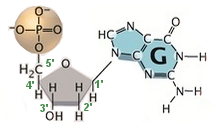
\includegraphics[width=0.5\textwidth]{nucleotideo.png}
    \caption{Nucleotídeo com grupo fosfato (P), pentose abaixo à esquerda e base nitrogenada G (no caso a Guanina). Adaptado de \cite{dnadiscovery08}. }
    \label{fig:Nucleotideo}
\end{figure} 

\indent Na Figura \ref{fig:Nucleotideo}, observa-se que no nucleotídeo existe uma numeração de 1' à 5', que representam os carbonos presentes na pentose. Para a criação de uma fita de ácido nucleico, existe uma ligação entre o carbono da posição 5' de um nucleotídeos e o carbono de posição 3' de outro \cite{setubal97}. Por definição o sentido da leitura de uma fita de ácido nucleico é 5' $\rightarrow$ 3', o que deve ser levado em consideração ao se fazer interpretação de dados do material genético.

\indent Dois tipos de ácidos nucleicos são encontrados nos seres vivos: ácido desoxirribonucleico (ADN) e ácido ribonucleico (ARN). Eles diferenciam-se na estrutura das bases nitrogenadas e em suas funções. O ADN é formado por uma desoxirribose, indicada na figura \ref{fig:EstruturasDoDNA}. Cada nucleotídeo de uma fita liga-se a partir de suas bases nitrogenadas com um nucleotídeo de outra fita, formando assim um eixo helicoidal tridimensional chamada de dupla hélice \cite{setubal97}. Esta ligação é feita entre grupos de purinas\footnote{composto orgânico que possui um anel duplo de carbono.}, Adenina (A) e Guanina (G), e pirimidinas\footnote{composto orgânico que possui um anel simples de carbono.}, Timina (T) e Citosina (C). Já o ARN possui apenas uma fita, onde a Timina (T) é substituída pela Uracila (U).

\indent O ADN é uma biomolécula que armazena as informações referentes ao funcionamento de todas as células dos seres vivos. Uma fita de ADN pode conter centenas de milhões de nucleotídeos. A representação do ADN, seja nos livros ou computacionalmente, é dada por um par em paralelo de strings de letras A, T, G e C. Como explicado no início dessa seção, o sentido padrão da leitura de uma fita é de 5' $\rightarrow$ 3', e no caso do ADN, as hélices são dispostas de maneira antiparalela, ou seja, uma é lida de 5' $\rightarrow$ 3' e a outra, de 3' $\rightarrow$ 5'. Observa-se que a partir de uma hélice, pode-se inferir a sequência de sua hélice complementar. Por exemplo, seja uma hélice H1 igual a AGTAAGC; então H2 em seu sentido oposto é H2' igual a TCATTCG, e no sentido biológico, igual a GCTTACT. A Figura \ref{fig:EstruturasDoDNA} apresenta a estrutura do ADN como explicada nesta seção.

\indent O ARN é uma biomolécula que possui diversas funções nas células dos organismos. Existem três tipos de ARNs presentes no citoplasma \footnote{espaço entre a membrana plasmática e o núcleo da célula.}. Cada um possui funções específicas que serão detalhadas na Seção \ref{sinteseDeProteina}. De maneira resumida, o ARN mensageiro (mARN) é responsável pela transferência de informação do ADN. Em seguida o ARN ribossômico (rARN) será combinado com o ARN transportador (tARN) para realizar a síntese de proteína.

\begin{figure}[h]
    \centering
    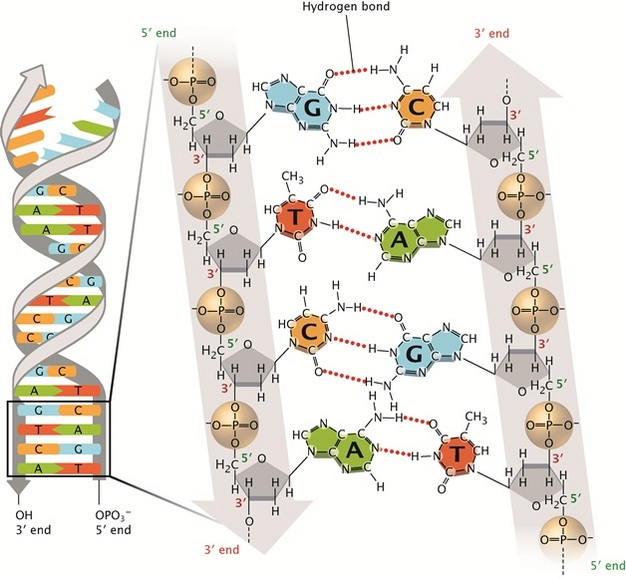
\includegraphics[width=0.7\textwidth]{dnaEstrutura.jpg}
    \caption{Representação das duas fitas de ADN, que se ligam por pontes de hidrogênio entre os nucleotídeos. Adaptado de \cite{dnadiscovery08}.}
    \label{fig:EstruturasDoDNA}
\end{figure} 


%% ================================================================================================================== %%

\subsection{Proteínas} \label{proteinas}

\indent As proteínas são biomoléculas com diversas funcionalidades nas células dos seres vivos. As proteínas fibrosas, como o colágeno, compõem a estrutura do corpo e para isso precisam ser resistentes e insolúveis em água. As proteínas globulares, como a hemoglobina, posuem formato esférico e são compactas, o que as permite realizar processos dinâmico pelo corpo \cite{LauraProteinas07}. Cada tarefa é realizada por uma proteína com uma estrutura específica e adaptada pra tal.

\indent Assim como os ácidos nucleicos, as proteínas são polímeros, macromoléculas cujos monômeros são aminoácidos. Aminoácidos são moléculas que possuem cinco componentes: amina (NH$_{2}$), carbono (C), hidrogênio (H), ácido carboxílico (COOH) e uma cadeia lateral que funciona como identificador de cada um dos 20 tipos de aminoácidos presentes nos seres vivos. A maneira como eles são criados será explicada com mais detalhes em seguida, pois envolve um processo complexo de síntese de proteína. A ligação, ou polimerização, de dois aminoácidos é feita unindo o grupo amino de um com o ácido carboxílico do outro, liberando uma molécula de água (H$_{2}$O) e formando uma cadeia chamada de dipeptídeo. Como houve liberação de água na ligação, o dipeptídeo não é formado por aminoácidos, mas sim resíduos dos mesmos. Nesse sentido, cadeias peptídicas de 100 à 5000 diferentes resíduos aminoácidos, ou cadeia polipeptídicas,  constituem a proteína.

\indent Existem quatro estruturas para caracterização de uma proteína \cite{setubal97}, apresentadas na Figura \ref{fig:EstruturasDaProteina}. A mais simples é chamada de estrutura primária e é composta por uma sequência linear de resíduos aminoácidos. A estrutura secundária é tridimensional e estabiliza-se por meio de ligações de hidrogênio na cadeia principal, chamada de \textit{backbone}. Dependendo da disposição dos resíduos de aminoácidos, esta cadeia pode se dar forma de hélice ($\alpha$-Helix) ou em forma de folha ($\beta$-Helix). A estrutura terciária é dada pela união de várias estruturas secundárias e, por fim, a estrutura quaternária é composta de múltiplas estruturas terciárias \cite{drug09}.

\begin{figure}[h]
    \centering
    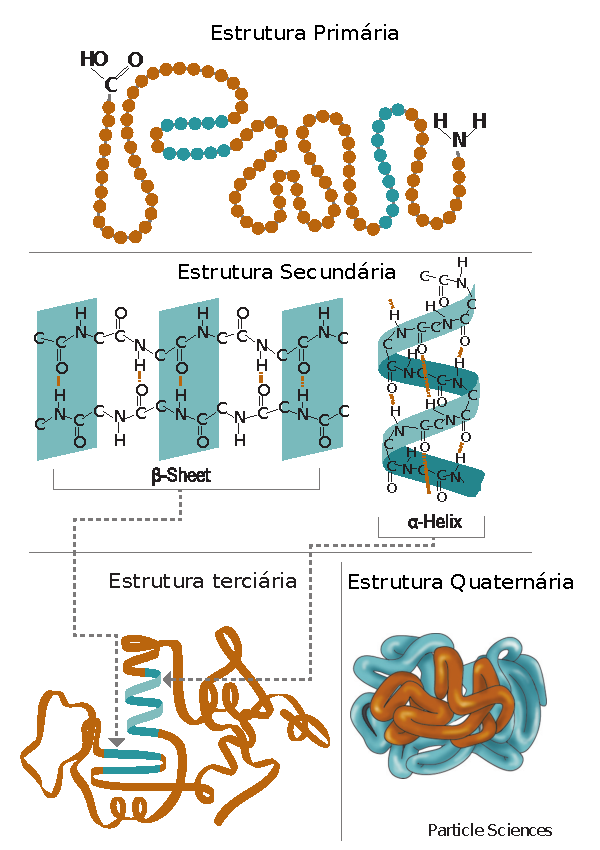
\includegraphics[width=0.6\textwidth]{EstruturasDaProteina.pdf}
    \caption{Quatro estruturas de proteínas. As unidades esféricas na estrutura primária representa os aminoácidos da proteína. Adaptado de \cite{drug09}.}
    \label{fig:EstruturasDaProteina}
\end{figure}

\subsection{Síntese de Proteína} \label{sinteseDeProteina}
% PROCARIÓTAS
\indent A \textbf{transcrição} é o processo de produção de mARN a partir do ADN e ele ocorre da seguinte forma: O início de cada gene possui um identificador em uma das fitas para indicar o local da codificação e, a partir dali, uma cópia inversa (A, T, C, G são traduzidos para U, A, G, C respectivamente) do mesmo é feita sob forma de molécula de mARN que, por consequência, obterá a mesma sequência que a cadeia codificadora (a qual não possui o identificador), porém trocando o U por T.

\indent O mARN deixa, então, o núcleo celular e inicia a \textbf{tradução} no citoplasma. O processo ocorre no interior de uma organela celular chamada de ribossomo, constituído de proteínas e rARN e cuja função é construir a molécula de proteína a partir de duas entradas, o mARN e tARN. A estrutura do tARN é tal que de um lado se encaixa exatamente um códon\footnote{Sequência de três nucleotídeos.} e no oposto, seu aminoácido correspondente, conforme ilustrado na Figura \ref{fig:sinteseProteina}. O processo de tradução se dá da seguinte forma: à medida em que o mARN passa pelo interior do ribossomo, este atrai quaisquer tARNs das proximidades cujos códons sejam correspondentes ao da subsequência corrente do mARN. No momento em que o códon do tARN conecta-se com um dos códons do mARN, a molécula de proteína em desenvolvimento é liberada e, com o auxílio da catálise de uma enzima, agregada no aminoácido que estava fixado naquele tARN. A tabela contendo a tradução de códon para aminoácido é fixa e chama-se código genético, apresentado na Tabela \ref{tabelaCodigoGenetico}. A tradução é finalmente completa quando o mARN apresenta um códon de parada, pois nenhum tARN possui correspondência para tal \cite{setubal97}. Uma proteína simples é, então, formada. 

\begin{figure}[h]
    \centering
    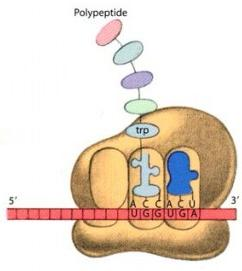
\includegraphics[width=0.35\textwidth]{sinteseProteina.png}
    \caption{Representação da etapa final da síntese de proteína, que sempre finaliza com o códon UGA. Adaptado de \cite{proteinSyntesis}.}
    \label{fig:sinteseProteina}
\end{figure} 


\begin{table}[h!] 
\centering
%\captionsetup{labelsep=space,justification=justified,singlelinecheck=off}
\caption{Código Genético que mapeia cada códon à um dos 20 aminoácidos, representados de maneira abreviada.} \label{tabelaCodigoGenetico}
\begin{tabular}{|c|c|c|c|c|c|c|c|}
\hline
 \multirow{2}{*}{ \begin{tabular}[x]{@{}c@{}} Primeira \\ Posição \end{tabular} } & 
 \multicolumn{4}{|c|}{Segunda Posição} & 
 \multirow{2}{*}{ \begin{tabular}[x]{@{}c@{}} Terceira \\ Posição \end{tabular} }\\  \cline{2-5}
 & G & A & C & U &  \\ \hline
 
 \multirow{5}{*}{G} & Gly & Glu & Ala & Val & G \\ 
 					& Gly & Glu & Ala & Val & A \\ 
 					& & & & & 					 \\ 
 					& Gly & Asp & Ala & Val & C \\ 
 					& Gly & Asp & Ala & Val & U \\ \hline 
 					
 \multirow{5}{*}{A} & Arg & Lys & Thr & Met & G \\ 
 					& Arg & Lys & Thr & Ile & A \\ 
 					& & & & & 					 \\ 
 					& Ser & Asn & Thr & Ile & C \\ 
 					& Ser & Asn & Thr & Ile & U \\ \hline 
 					
 \multirow{5}{*}{C} & Arg & Gln & Pro & Leu & G \\ 
 					& Arg & Gln & Pro & Leu & A \\ 
 					& & & & & 					 \\ 
 					& Arg & His & Pro & Leu & C \\ 
 					& Arg & His & Pro & Leu & U \\ \hline 
 					
 \multirow{5}{*}{U} & Trp & \textbf{FIM} & Ser & Leu & G \\ 
 					& \textbf{FIM} & \textbf{FIM} & Ser & Leu & A \\ 
 					& & & & & 					 \\ 
 					& Cys & Tyr & Ser & Phe & C \\ 
 					& Cys & Tyr & Ser & Phe & U \\ \hline 
 
\end{tabular}
\end{table}

%% ================================================================================================================== %%


\section{Conceitos Básicos de Metabolismo} \label{conceitosMeta}


% metabolismo

% via metabólica

% rede metabólica

\indent As proteínas podem ser enzimas, macromoléculas responsáveis por auxiliar a realização de biossíntese (construção) e biodegradação de moléculas no metabolismo. As enzimas têm o propósito de catalisar, ou acelerar, reações bioquímicas que naturalmente levariam muito mais tempo para serem realizadas no organismo \cite{setubal97}. Geralmente as enzimas catalisam uma reação específica e seus nomes correspondem à tarefa que elas executam com adição do sufixo "ase". Por exemplo, a Sintetase realiza biossíntese, a Desidrogenases realiza oxi-redução (transferência de elétrons) e a Quinase transporta elementos químicos de uma molécula para outra \cite{enzymesKirk}.

\indent As reações bioquímicas são alterações químicas que fornecem um ou mais produtos a partir de um ou mais substratos \cite{lacroixCTS08}. Esses produtos e substratos são compostos químicos chamados de metabólitos. A presença de um metabólito em um certo local de um organismo depende do tipo de célula e do tipo de compartimento em que ele se encontra dentro da célula. Normalmente as reações ocorrem em apenas uma direção, ou seja, os produtos não pode gerar os substratos de uma mesma reação \cite{lacroixCTS08}.

\indent Ao catalisar uma reação, uma enzima possue comportar um ou mais substratos em um local pré-determinado em formato côncavo chamado de sítio ativo. Se ela comporta apenas um substrato, a estrutura que se forma com o preenchimento do sítio ativo é um complexo enzima-substrato. Porém se ela comporta mais de um substrato, a estrutura é chamada de complexo ternário intermediário \cite{Cap2schomburg}. Duas enzimas ainda podem possuir a mesma atividade enzimática porém apresentar estruturas físicas diferentes. Essas são chamadas isoenzimas \cite{Cap2schomburg}.

\indent Dentro das células existem também pequenas moléculas que regulam (aumentam ou diminuem) as atividades enzimáticas, chamados cofatores. Eles são componentes químicos não-proteicos e podem ser orgânicos ou inorgânicos \cite{lacroixCTS08}. Cofatores podem ser coenzimas, associadas momentaneamente às enzima, ou grupos prostéticos, associados firmemente à elas \cite{Cap2schomburg}.

\indent Uma sequência de reações bioquímicas é chamada de via metabólica. As vias metabólicas podem ser anabólicas (realizam síntese de moléculas complexas gastando energia) ou catabólicas (realizam a quebra de moléculas complexas produzindo energia) \cite{lacroixCTS08}. Geralmente a energia liberada pelas reações catabólicas é usada para impulsionar as reações anabólicas \cite{carterClass}. A Figura \ref{fig:bioLuz} apresenta um exemplo de via metabólica, a bioluminescência de uma bactéria. Ela possui oito reações, quatro produtos intermediários e um produto final, que é um photon (luz).

\begin{figure}[h]
    \centering
    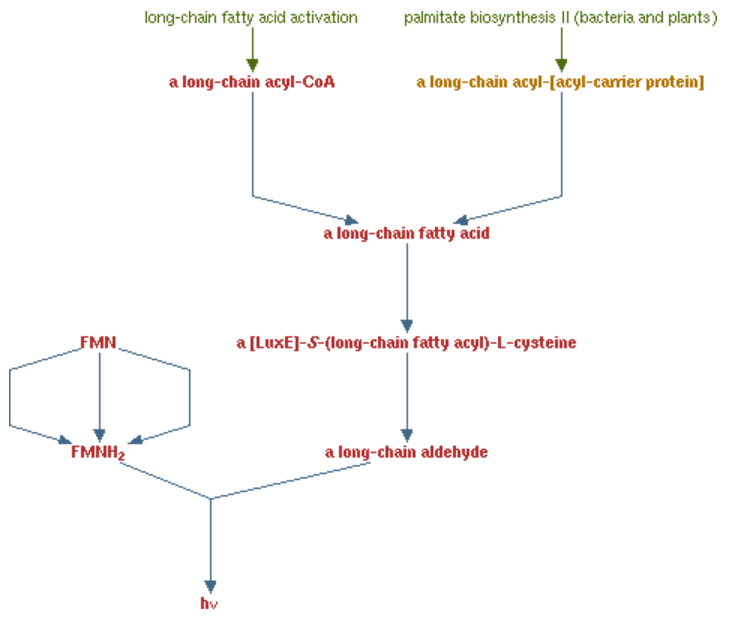
\includegraphics[width=0.7\textwidth]{bioLuz.png}
    \caption{Exemplo de via metabólica retirado do site MetaCyC. Esta representa o processo de produção da bioluminescência de bactérias \cite{examplePathway}. }
    \label{fig:bioLuz}
\end{figure}

\indent O conjunto de todas as vias metabólicas de um determinado organismo é chamado de rede metabólica. Pesquisadores de Biologia Molecular podem analisar tanto as vias metabólicas separadamente quanto em conjunto, avaliando as interações entre elas dentro de uma rede metabólica \cite{lacroixCTS08}. Uma das vantagens de se estudar as vias em conjunto é poder explorar vias alternativas para um mesmo fim biológico \cite{lacroixCTS08}.

\subsection{Metabolismo Primário}

\indent O metabolismo, além de ser subdivido em catabolismo e anabolismo, também pode ser classificado em relação à função que exerce no organismo. Se a função realizada é fundamental no organismo, como crescimento, desenvolvimento e reprodução, ele é denominado metabolismo primário \cite{Cap3schomburg}. São exemplos de metabolismos primários os processos de divisão celular mitose e meiose, a primeira para crescimento e a segunda para reprodução, conforme indicado na Figura \ref{fig:mitoseEmeiose}.

\begin{figure}[h]
    \centering
    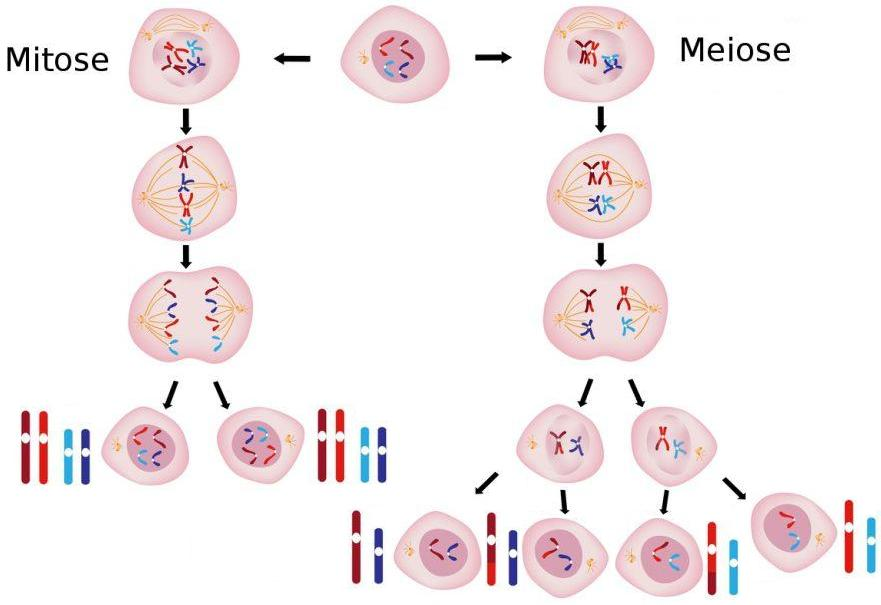
\includegraphics[width=0.5\textwidth]{mitoseEmeiose.jpg}
    \caption{A célula que se divide por meio de mitose gera duas outras células idênticas à original. A célula que se divide por meio de meiose gera quatro células, cada uma com metade do material genético da célula original. Adaptado de \cite{mitoseMeiose}. }
    \label{fig:mitoseEmeiose}
\end{figure} 

\subsection{Metabolismo Secundário}

\indent No caso dos metabolismos que não realizam função essencial no organismo, eles são classificados como metabolismos secundários. Esses são caracterizados pela vasta diversidade química e, desta forma, são responsáveis pela sobrevivência do organismo em diferentes meio ambientes de acordo com os fatores bióticos (elementos causados pela interação entre organismos como, por exemplo, cadeia alimentar) e abióticos (elementos naturais independente de organismos como, por exemplo, luz e temperatura) \cite{Cap3schomburg}.

\indent Enquanto 20\% dos metabólitos secundário são encontrados em bactérias, fungos e organismos sésseis\footnote{Que vivem fixos, sem capacidade de locomoção.} marinhos, os outros 80\% encontram-se em plantas vasculares\footnote{QUE PORRA EH ESSA *****} \cite{Cap3schomburg} e esses podem ser subdivididos em três classes: terpenóides, alcaloides e fenólicos \cite{kabera14}. A seguir está uma breve explicação de cada uma dessas classe, acompanhada da Figura \ref{fig:metSecundario} que apresenta um exemplo de composto químico para cada grupo.

\begin{itemize}
\item Os \textbf{terpenóides} constituem no grupo mais abundante de produtos naturais, apresentando uma grande variedade estrutural e funcional, principalmente no Reino \textit{Plantae}. No metabolismo secundário, possuem funções como produção de óleos, esteroides, cera, resinas e borracha natural, produção de compostos usados para defesa contra herbívoros ou aromas usados para atrair polinizadores \cite{Cap3schomburg};

\item Os \textbf{alcaloides} são majoritariamente tóxicos a outros organismos diferentes daquele que os produz. Nesse sentido, eles possuem nas plantas função de defesa contra herbívoros e podem ser encontrados principalmente nos locais mais propícios à ataques, por exemplo, nas sementes, flores e tecidos periféricos em crescimento. Para o consumo dos seres humanos, são usados na fabricação de estimulantes, como cafeína e nicotina, e drogas, como morfina \cite{Cap3schomburg}. Por apresentarem alta diversidade estrutural, é difícil classificá-los. A tentativa mais recente baseia-se na semelhanças entre os esqueletos carbônicos \cite{kabera14};

\item Os \textbf{fenólicos} são caracterizados por suas propriedades anti-oxidantes, anti-inflamatórias e anti-cancerígenas e muitos deles são bactericidas, antissépticos e vermífugos. Eles estão presentes em praticamente todas as plantas e são utilizados na Química, Biologia, Agricultura e Medicina \cite{kabera14}.
\end{itemize}

\begin{figure}[h]
    \centering
    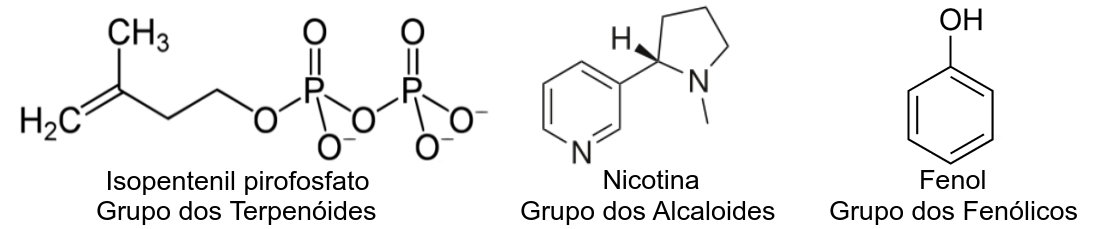
\includegraphics[width=0.8\textwidth]{metSecundario.png}
    \caption{Um exemplo de elemento químico para cada classe, ou grupo, de metabolismo secundário.}
    \label{fig:metSecundario}
\end{figure} 

%% ================================================================================================================== %%

\section{Visualização de Redes Metabólicas} \label{BDredes}


% Surgimento de bancos de dados (PAM, GenBank)

\indent Desde o descobrimento da estrutura do ADN por Crick e Watson, o número de sequências de proteínas descobertas cresceu, aumentando também a necessidade de serem criados bancos de dados para armazená-las. A físico-química norte-americana Margaret Dayhoff, com colaboração de alguns membros do \textit{National Biomedical Research Foundation} em Washington, foi a primeira a construir um banco de dados com este propósito em um tipo de atlas de proteínas na década de 60 \cite{mount01}. Somente em 1984 esta coleção foi intitulada de \textit{Protein Information Resource} \cite{mount01}. Os dados eram organizados de acordo com o grau de similaridade das sequências, onde o agrupamento das mesmas era dado em forma de árvore filogenética representando famílias e superfamílias de proteínas. Caso a semelhança fosse alta, é provável que elas teriam as mesmas funções bioquímicas e estrutura tridimensional.

\indent A partir da árvore gerada, foi possível calcular as mutações que ocorreram nos aminoácidos durante a evolução genética e, então, produzir uma tabela utilizada até hoje, chamada PAM (\textit{Percent Acept Mutation}), que apresenta tais dados\footnote{1 PAM é uma medida de tempo para representar 1 mutação para cada 100 aminoácidos.}. Hoje em dia também utiliza-se uma outra matrix, chamada BLOSUM (\textit{Block Substitution Matrix}), que, ao contrário da PAM que identifica as semelhanças entre sequências de proteínas, identifica a divergência evolucionária entre sequências de proteínas.

\indent Outro banco de dados de grande porte e bastante utilizado nos dias de hoje é o \textit{GenBank}, criado em 1982 por Walter Goad e demais colaboradores com o objetivo de catalogar sequências genéticas e coleções de anotações de todos os ADNs públicos, agora, com o patrocínio do \textit{National Center for Biotechnology Information} (NCBI). Os dois bancos são públicos e continuam crescendo exponencialmente \cite{mount01}. 

% Especificar banco de dados para Redes metabólicas

\indent Nos dias de hoje, a quantidade de dados é tão grande e  que os biólogos enfrentam dificuldades em tarefas como análise, busca, armazenamento, visualização e atualização de dados. Nesse sentido, eles utilizam agora ferramentas de Big Data em suas pesquisas. Existem grandes áreas da Biologia Molecular voltadas para estudo desse dados (chamados de dados ômicos), tais como, por exemplo, genoma\footnote{Material genético de um organismo.}, transcritoma\footnote{Conjunto dos transcritos mARN, tARN, rARN e microARN.}, proteoma\footnote{Conjunto de proteínas e suas variantes em um organismo.}, metaboloma\footnote{Conjunto de metabólitos de um organismo.} e interactoma\footnote{Conjunto de interações moleculares em um organismo.}.

\indent Nesta seção serão apresentados quatro grandes bancos de dados utilizados no estudo do metaboloma (Reactome, KEGG, MetaCyc e 2Path), bem como seus sistemas de visualização de dados. O foco será dado ao 2Path, sistema desenvolvido neste projeto. 
%
% This kind of database is however an exception among genome-scale metabolic databases. Besides being often much less accurate, most of the pathways in BioCyc or in KEGG, another widely used database for metabolism [7], are further biased towards the microbial and plant kingdoms. The quality of the metabolic reconstruction of any animal is thus expected to be worse than the one of a bacterium evolutionarily close to Escherichia coli.
%
% \cite{lacroixCTS08}

%\textbf{Banco de Dados NoSQL}

%\indent Para comportar tamanha quantidade de dados e ao mesmo tempo providenciar alta performance, atualmente é possível utilizar um banco de dados NoSQL como alternativa ao tradicional modelo relacional. NoSQL pode significar Não-Relacional ou \textit{Not Only SQL}  \cite{cattell11}, para ressaltar as vantagens sobre o modelo tradicional, que são rápida leitura e escrita dos dados, suporte à armazenamento em larga escala, fácil escalabilidade, fácil distribuição (replicação ou fragmentação) de dados entre vários servidores, e baixo custo. \cite{jing12}. Entretanto, uma grande desvantagem é sua falta de suporte à linguagem SQL, o que obriga o usuário a aprender a recuperar seus dados de outra maneira\footnote{No banco de dados Neo4j, por exemplo, usa-se a linguagem CYPHER.}.

%\indent Em 2000, o Professor Eric Brewer da Universidade da Califórnia em Berkeley estabeleceu o Teorema CAP (\textit{Consistency, Availability and Partition tolerance}), que afirma que quando os dados estão particionados\footnote{Falha em algum dispositivo de rede que causa a separação entre dois conjuntos de computadores.} em rede, os BDs NoSQL que são distribuídos devem tolerar tal falha e oferecer, assim, apenas duas escolhas para o usuário: consistência ou disponibilidade de dados, nunca os dois ao mesmo tempo. \cite{jing12} \cite{cattell11}. Caso o banco decida fornecer mais consistência do que disponibilidade, o sistema tentará sempre retornar a \textit{query} com dados atualizados para o usuário, mesmo que a operação demore. A Figura \ref{fig:capTheorm} ilustra o teorema também conhecido como Teorema de Brewer. Caso decida fornecer mais disponibilidade do que consistência, o sistema tentará retornar a \textit{query} o mais rápido possível, mesmo se o dados estiverem desatualizados. Esta \textit{trade-off} inerente na maioria dos BDs NoSQL pode, na verdade, ser decidida pelo próprio usuário ao configurar seu banco de dados. \\ 

%\begin{figure}[h]
%    \centering
%    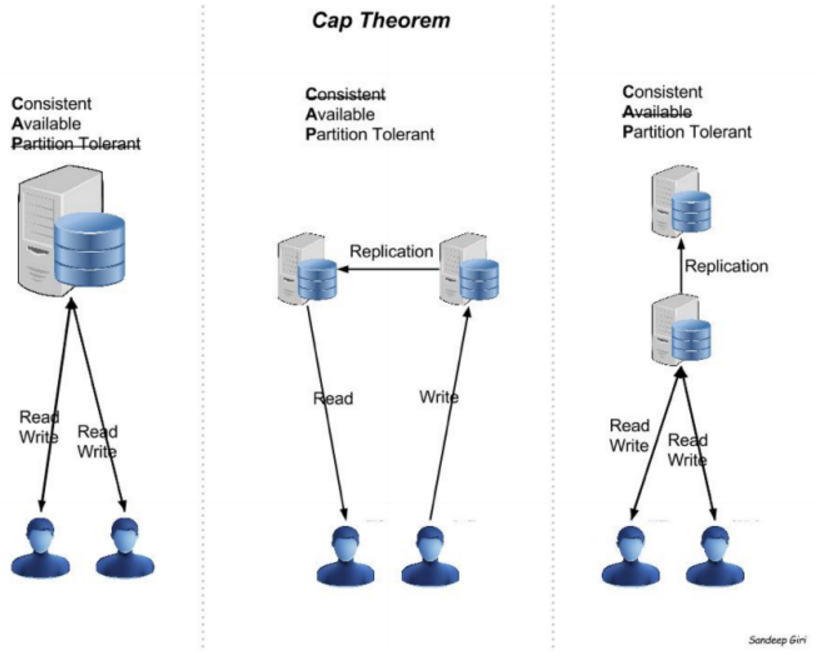
\includegraphics[width=0.8\textwidth]{capTheorm.png}
%    \caption{Teorema CAP. Na primeira coluna, o banco de dados não suporta partição de rede, na segunda existe replicação parcial de dados entre os servidores e na terceira, replicação total \cite{CAPTheorem}.}
%    \label{fig:capTheorm}
%\end{figure} 

%\textbf{Banco de Dados em Grafo}

%\indent Grafos são as estruturas mais úteis para se representar interações entre objetos, portanto são de grande interesse no campo biológico, na modelagem de dados ômicos \cite{vicknair10}. Bancos de dados em grafo podem ser utilizados, por exemplo, quando a finalidade é buscar via \textit{query} a procedência dos objetos\footnote{A procedência é a linhagem do dado, ou seja, os detalhes de sua criação desde a origem conhecida.}, pois realizar uma travessia em grafo é bem mais rápido computacionalmente do que realizar múltiplos \textit{JOINS} num modelo relacional.

%\indent Ao se trabalhar com banco de dados em grafos, é importante ter conhecimento das principais terminologias a seguir:
%\begin{itemize}
%\item Adjacência: Nós que dividem uma aresta incidente ou arestas que dividem um nó incidente;
%\item Aresta: Uma registro que representa relação entre um par de objetos. Pode possuir direção, quando a relação possui origem e destino, ou não;
%\item Caminho: Coleção de alternados nós e arestas;
%\item \textit{Constraint}: Restrição definida pelo usuário que o banco deve impor aos dados;
%\item DAG: Um grafo direcionado e acíclico;
%\item Incidência: Aresta adjacente associada à um nó, ou nó associado à uma aresta;
%\item \textit{Label}: Rótulo de um nó que o agrupa em algum subconjunto; 
%\item \textit{Loop}: Uma aresta que conecta um nó à ele mesmo;
%\item Nó: Um registro que representa um objeto e possui um número indefinido de propriedades, labels e arestas incidentes;
%\item Propriedade: Atributo armazenado em um nó ou aresta;
%\item Registro: Unidade de armazenamento;
%\item Vizinho: Nó conectado por uma aresta em comum.
%\end{itemize}

% ____________________________________________________________________
% ____________________________________________________________________
% ____________________________________________________________________

\subsection{Reactome}

\indent Reactome\footnote{Disponível pela \textit{web}, em \url{http://www.reactome.org}.} é um banco de dados de reações de mudança de estado, ou seja, além de reações bioquímicas, ele também abrange reações de ativação, de degradação e de ligação, por exemplo \cite{reactomeUsersguide}. Ele faz uma ligação sistemática entre as proteínas de um certo organismo e as funções moleculares do mesmo, fornecendo uma base de funções que pode ser utilizada para pesquisas sobre expressão de genes ou mutações somáticas. 
\indent O Reactome disponibiliza o \textit{Pathway Browser}, uma rede geral para cada organismo, que representa os vários seus sistemas, como reprodução e metabolismo, por exemplo. Algumas sub-redes estão conectadas (por exemplo, replicação de ADN e ciclo de célula), outra não (por exemplo, contração muscular e reprodução). 

\indent Nesta rede, cada nó representa uma via cujo número de entidade se reflete no raio do nó, e cada aresta representa a relação entre estas vias. A página ainda possui uma ferramenta de análise de dados baseada nas correspondências entre as reações na redes dos organismos comparados.

\indent Para acessa sua ferramenta de visualização, basta navegar a partir da \textit{home page}:

\indent \colorbox{yellow}{\url{http://www.reactome.org/} $\Rightarrow$} \\
\indent \colorbox{yellow}{Browse Pathways} \\

\begin{figure}[!h]
\centering
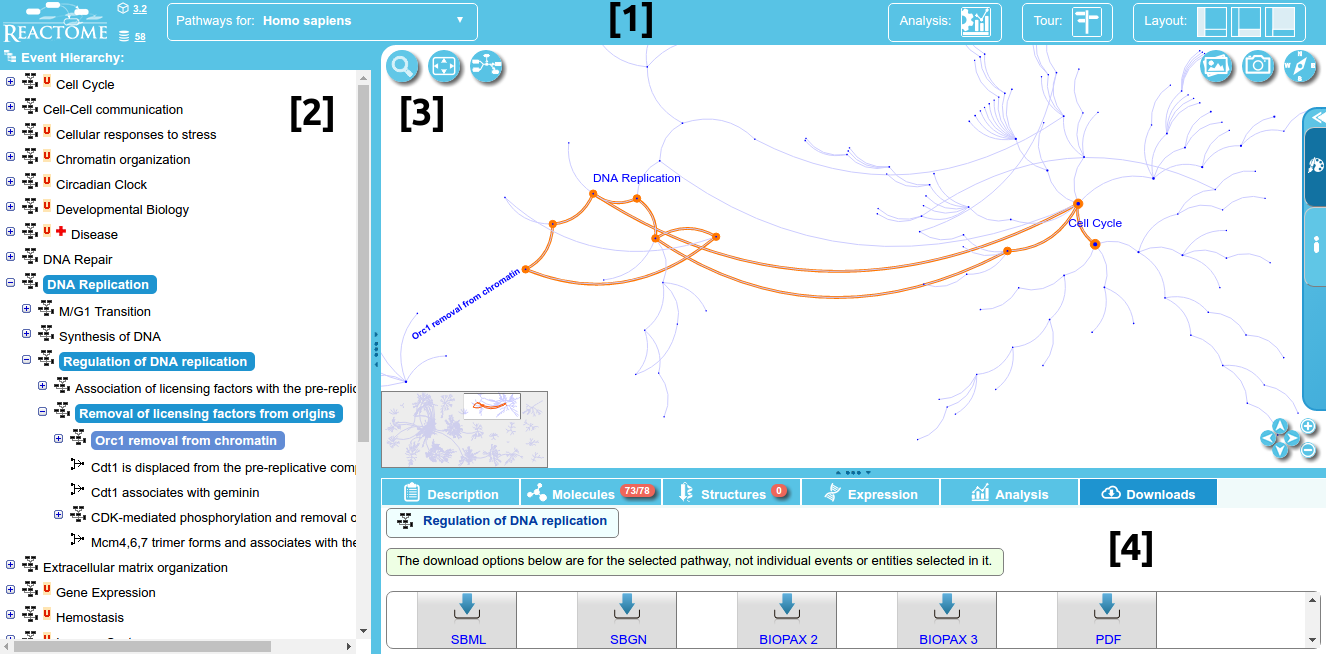
\includegraphics[width=1\textwidth]{reactomeBrowser_idBW.png}
\caption{Visão geral da rede metabólica do \textit{Homo sapiens} do Reactome, com destaque na via metabólica de remoção do Orc1 da cromatina do processo de regulação da replicação do ADN. A interface pode ser dividida nas seções [1], [2], [3] e [4].}
\label{reactomeBrowser_id}
\end{figure}

\indent Segue abaixo a descrição de cada elemento da interface da ferramenta de visualização do Reactome, subdivididos  conforme indicado na Figura \ref{reactomeBrowser_id}.

\begin{itemize}
\item[[ 1]] Menu de navegação direta e indiretamente relacionado às vias metabólicas. À esquerda tem-se a versão do \textit{Pathway Browser} e de seu banco de dados e um menu \textit{dropdown} para se selecionar o organismo mostrado na interface. À direita tem-se um \textit{link} (\textit{Analysis}) para a uma página modal onde é possível analisar os dados do usuário e fazer comparação entre espécies, um \textit{link} (\textit{Tour}) para um vídeo explicando como \textit{Pathway Browser} funciona e um conjunto de \textit{layouts} que alteram a visualização geral da página;
\item[[ 2]] Lista de redes metabólicas ordenadas alfabeticamente;
\item[[ 3]] Mapa gerada em forma de grafo interativo. Quando uma rede metabólica da lista [2] é selecionada, ela se destaca no mapa. No topo, à esquerda é possível buscar por palavras chaves no mapa e visualizá-lo em tela cheia e à direita é possível visualizar imagens detalhadas das redes metabólicas, capturar uma imagem do mapa gerado e ler sobre a notação utilizada na página. Abaixo, à esquerda tem-se um mini-mapa por onde o usuário pode se localizar no mapa geral e à direita tem-se botões com o mesmo propósito e mais dois: (+) \textit{Zoom in} e (-) \textit{Zoom out}. Por fim, à direita do mapa existe um painel que se abre da direita para a esquerda que permite que o usuário edite as cores do mapa e obtenha informação sobre o mesmo.
\item[[ 4]] Menu de operação e informações sobre as redes metabólicas selecionadas em [2]. O \textit{Description} contém seus detalhes tais como compartimento celular e referências externas. O \textit{Molecules} contém uma lista de compostos químicos e proteínas associadas às vias. O \textit{Structures} oferece uma lista de imagens que representam a via e seus componentes. O Expression apresenta detalhes sobre o local no organismo onde ocorrem as reações das vias selecionadas. O \textit{Analysis} apresenta o resultado das análise feita em [1]. Finalmente o botão Downloads oferece arquivos das vias para baixar em diversos formatos tais como SBML e PDF. 
\end{itemize}

\indent Caso o usuário queira visualizar a(s) via(s) metabólica detalhadamente, basta clicar nos nós do mapa, cujo tamanho está diretamente relacionado ao número de entidades que compõem a via. A imagem do grafo desaparece e então um conjunto dos elementos que o compõe aparece em seu lugar. A Figura \ref{orcRemovalViaReactome} apresenta a via da remoção do Orc1 da cromatina do processo de regulação da replicação do ADN.

\begin{figure}[!h]
\centering
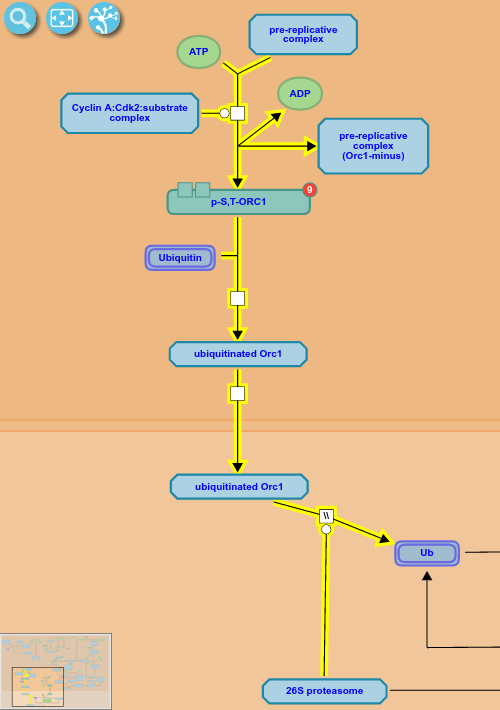
\includegraphics[width=0.7\textwidth]{orcRemovalViaReactome.png}
\caption{Via metabólica de remoção do Orc1 da cromatina apresentada pela ferramenta de visualização do Reactome.}
\label{orcRemovalViaReactome}
\end{figure}


% ____________________________________________________________________
% ____________________________________________________________________
% ____________________________________________________________________

\subsection{KEGG}

\indent O KEGG\footnote{Disponível pela \textit{web}, em \url{http://www.kegg.jp/}.} (\textit{Kyoto Encyclopedia of Genes and Genomes}) é uma base de informações sobre sistemas biológicos em nível molecular, sobretudo sobre conjuntos de dados em larga escala gerados por sequenciamento de genoma \cite{keggOverview}. 
\indent As informações sobre os sistemas podem ser dadas em forma de módulos, unidades funcionais com identificação otimizada para análise dos dados, em forma de \textit{brite}, coleção de arquivos estruturados hierarquicamente sobre as funções das entidades biológicos, ou em forma de vias, mapa de interações moleculares e reações químicas.
\indent Dado que o metabolismo é um conjunto de reações e transformações químicas, a maneira natural de representá-lo é por meio de uma rede de interações, ou seja, em forma de vias. O KEGG oferece uma ferramenta de busca de vias metabólicas sobre várias redes metabólicas, dos vários organismos que constituem o banco de dados.

\indent Para acessar sua ferramenta de visualização, basta navegar a partir da \textit{home page}: \\

\indent \colorbox{yellow}{\url{http://www.kegg.jp/} $\Rightarrow$} \\
\indent \colorbox{yellow}{Data-oriented entry points  $\mapsto$ KEGG PATHWAY $\Rightarrow$} \\
\indent \colorbox{yellow}{Pathway Maps $\mapsto$ 1. Metabolism  $\Rightarrow$} \\
\indent \colorbox{yellow}{1.0 Global and overview maps $\mapsto$ Metabolic pathways} \\

\begin{figure}[!h]
\centering
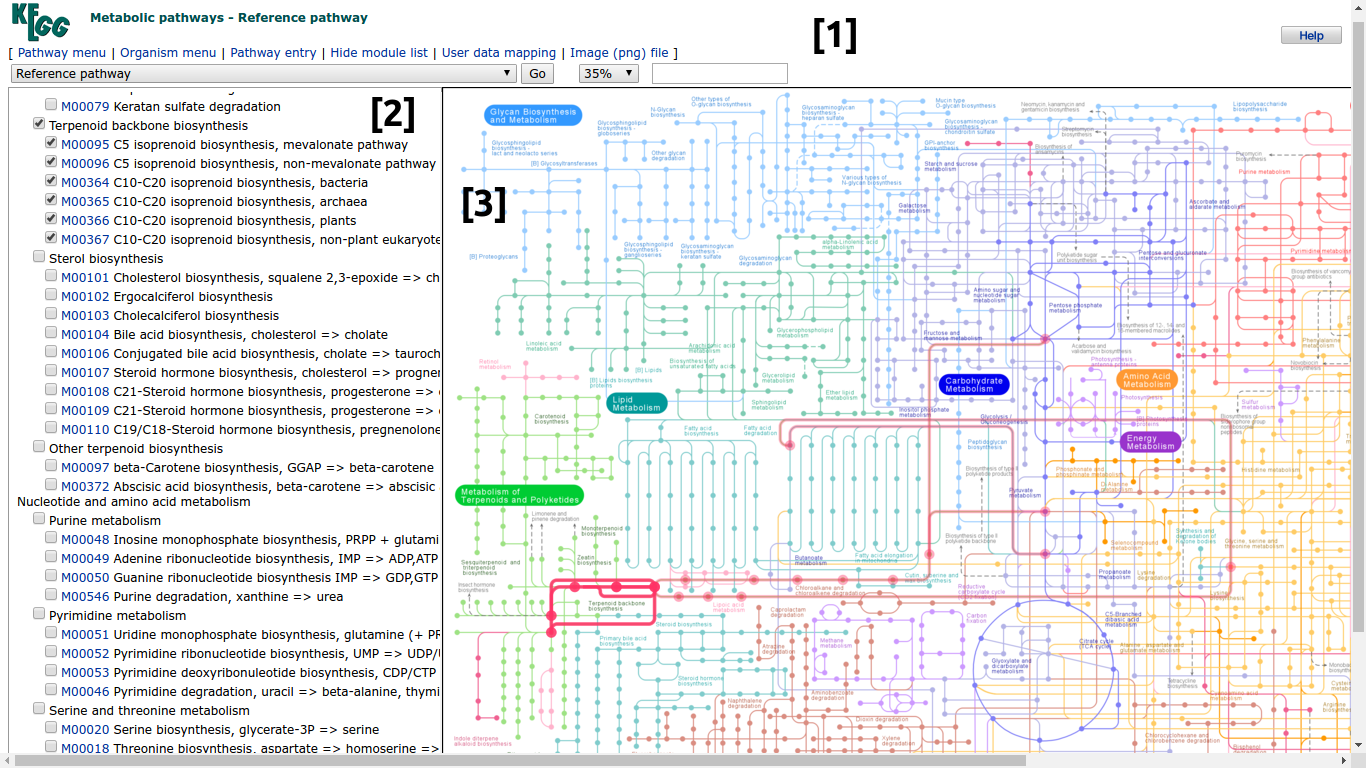
\includegraphics[width=1\textwidth]{terpenoidBackboneKEGG_idBW.png}
\caption{Visão geral da rede metabólica de referência do KEGG, com destaque na via metabólica de biossíntese do \textit{backbone} de terpenóides. A interface pode ser dividida nas seções [1], [2] e [3].}
\label{terpenoidBackboneKEGG_id}
\end{figure}

\indent Segue abaixo a descrição de cada elemento da interface da ferramenta de visualização do KEGG, subdivididos conforme indicado na Figura \ref{terpenoidBackboneKEGG_id}.

\begin{itemize}
\item[[ 1]] Menu de navegação direta e indiretamente relacionado às vias metabólicas. O \textit{Pathway menu} redireciona para uma página que contém uma lista \textit{links} para todos os diagramas mostrados no mapa geral. O \textit{Organism menu} redireciona para à uma página com uma lista de todos os organismos conhecidos pelo KEGG (346 eucariotas e 4159 procariotas\footnote{Visitado em 2016-10-06}). O \textit{Pathway entry} redireciona para a descrição da via metabólica selecionada. O \textit{Hide module list}, quando clicado, oculta a área [2] da página. O \textit{User data mapping} abre uma nova janela que solicita um objeto seguido de uma cor escolhida pelo o usuário para dar sua própria coloração às vias. Por fim, o \textit{Image (png) file} oferece a imagem do mapa para \textit{download}. Abaixo é possível escolher o organismo apresentado no mapa, sua resolução e buscar por palavras chaves;
\item[[ 2]] Lista de redes metabólicas organizadas de acordo com suas funções;
\item[[ 3]] Mapa gerada em forma de grafo interativo. Quando uma rede metabólica da lista [2] é selecionada, ela se destaca no mapa.
\end{itemize}

\indent Caso o usuário queira visualizar a(s) via(s) metabólica detalhadamente, o KEGG oferece uma lista de diagramas\footnote{Detalhes da notação dos diagramas: \url{http://www.genome.jp/kegg/document/help_pathway.html}} desenhados manualmente em formato de grafo interativo cujos nós, quando clicados, redirecionam para uma página contendo a descrição do objeto, que pode ser enzima, composto químico ou outra rele metabólica, por exemplo. Continuando com o exemplo da biossíntese do \textit{backbone} de terpenóides, para acessar seu diagrama, apresentado na figura \ref{terpenoidBackboneKEGG}, basta navegar a partir da \textit{home page}: \\

\indent \colorbox{yellow}{\url{http://www.kegg.jp/} $\Rightarrow$} \\
\indent \colorbox{yellow}{Data-oriented entry points  $\mapsto$ KEGG PATHWAY $\Rightarrow$} \\
\indent \colorbox{yellow}{Pathway Maps $\mapsto$ 1. Metabolism  $\Rightarrow$} \\
\indent \colorbox{yellow}{1.9 Metabolism of terpenoids and polyketides  $\mapsto$ Terpenoid backbone biosynthesis} \\

\begin{figure}[!h]
\centering
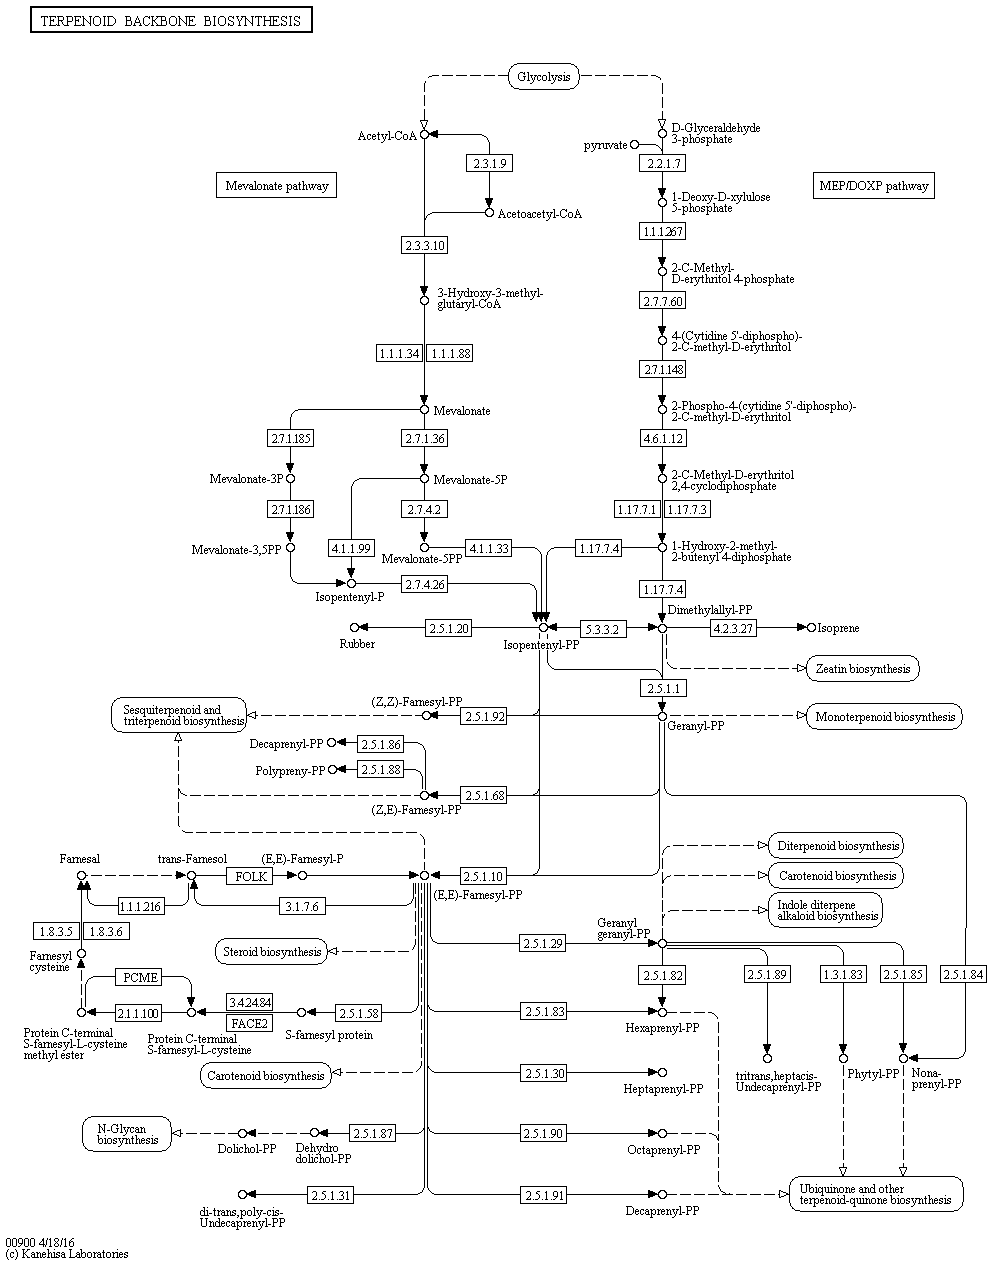
\includegraphics[width=1\textwidth]{terpenoidViaKEGG.png}
\caption{Via metabólica de biossíntese do \textit{backbone} de terpenóides apresentada pela ferramenta de visualização do KEGG.}
\label{terpenoidBackboneKEGG}
\end{figure}

% ____________________________________________________________________
% ____________________________________________________________________
% ____________________________________________________________________

\subsection{BioCyc}

\indent O BioCyc\footnote{Disponível pela \textit{web}, em \url{http://biocyc.org}.} é um sistema de coleção de aproximadamente 7 mil bancos de dados chamados PGDBs (\textit{Pathway/Genome Databases}) pois possuem duas maneiras diferentes de representar as informações: modelo de vias metabólicas, que enfatiza as sequências de reações, substratos e produtos de múltiplos organismos, ou modelo de sequência genômica, que destaca a localização e descrição dos genes de cada organismo específico \cite{biocycIntro}. 

\indent Os bancos PGDBs são organizado em três camadas de acordo com a frequência de atualizações/refinações e da maneira com que os dados foram obtidos. O BioCyc possui um banco de dados específico para redes metabólicas determinadas experimentalmente, chamado MetaCyc\footnote{Disponível pela \textit{web} através do site \url{http://metacyc.org/}.}. Este é o único banco de dados multi-organismos do grupo BioCyc e ele é referência na ferramenta gratuita \textit{Pathway Tools} desenvolvida pelo instituto de pesquisa \textit{SRI International}.

\indent Diferente das ferramentas do KEGG e Reactome, o Pathway  Tools não possui um mapa global de visualização das vias metabólicas. Para acessá-las, o usuário deve buscar por alguma palavra chave conhecida ou navegar pelo sumário de vias\footnote{Na última visita, em 2016-10-06, a página possuía 3.461 vias metabólicas.} classificado hierarquicamente com base em suas funções biológicas e na classe dos metabólitos produzidos\/consumidos. O acesso à via da Figura \ref{fig:bioLuz}, por exemplo, se deu pela navegação a partir da \textit{home page}: \\

\indent \colorbox{yellow}{\url{http://metacyc.org/} $\Rightarrow$} \\
\indent \colorbox{yellow}{Metabolism $\mapsto$ Browse Pathway Ontology $\Rightarrow$} \\
\indent \colorbox{yellow}{Pathways $\mapsto$ Bioluminescence (1 instances) $\mapsto$ bacterial bioluminescence} \\

\indent Cada nó das vias metabólicas quando clicado redireciona o usuário para uma página com mais detalhes sobre o objeto, que pode ser outra via, um composto químico ou uma enzima, por exemplo. A Figura \ref{bioLuz_id} é uma modificação da Figura \ref{fig:bioLuz} apresentando diretamente o conjunto destes elementos.

\begin{figure}[!h]
\centering
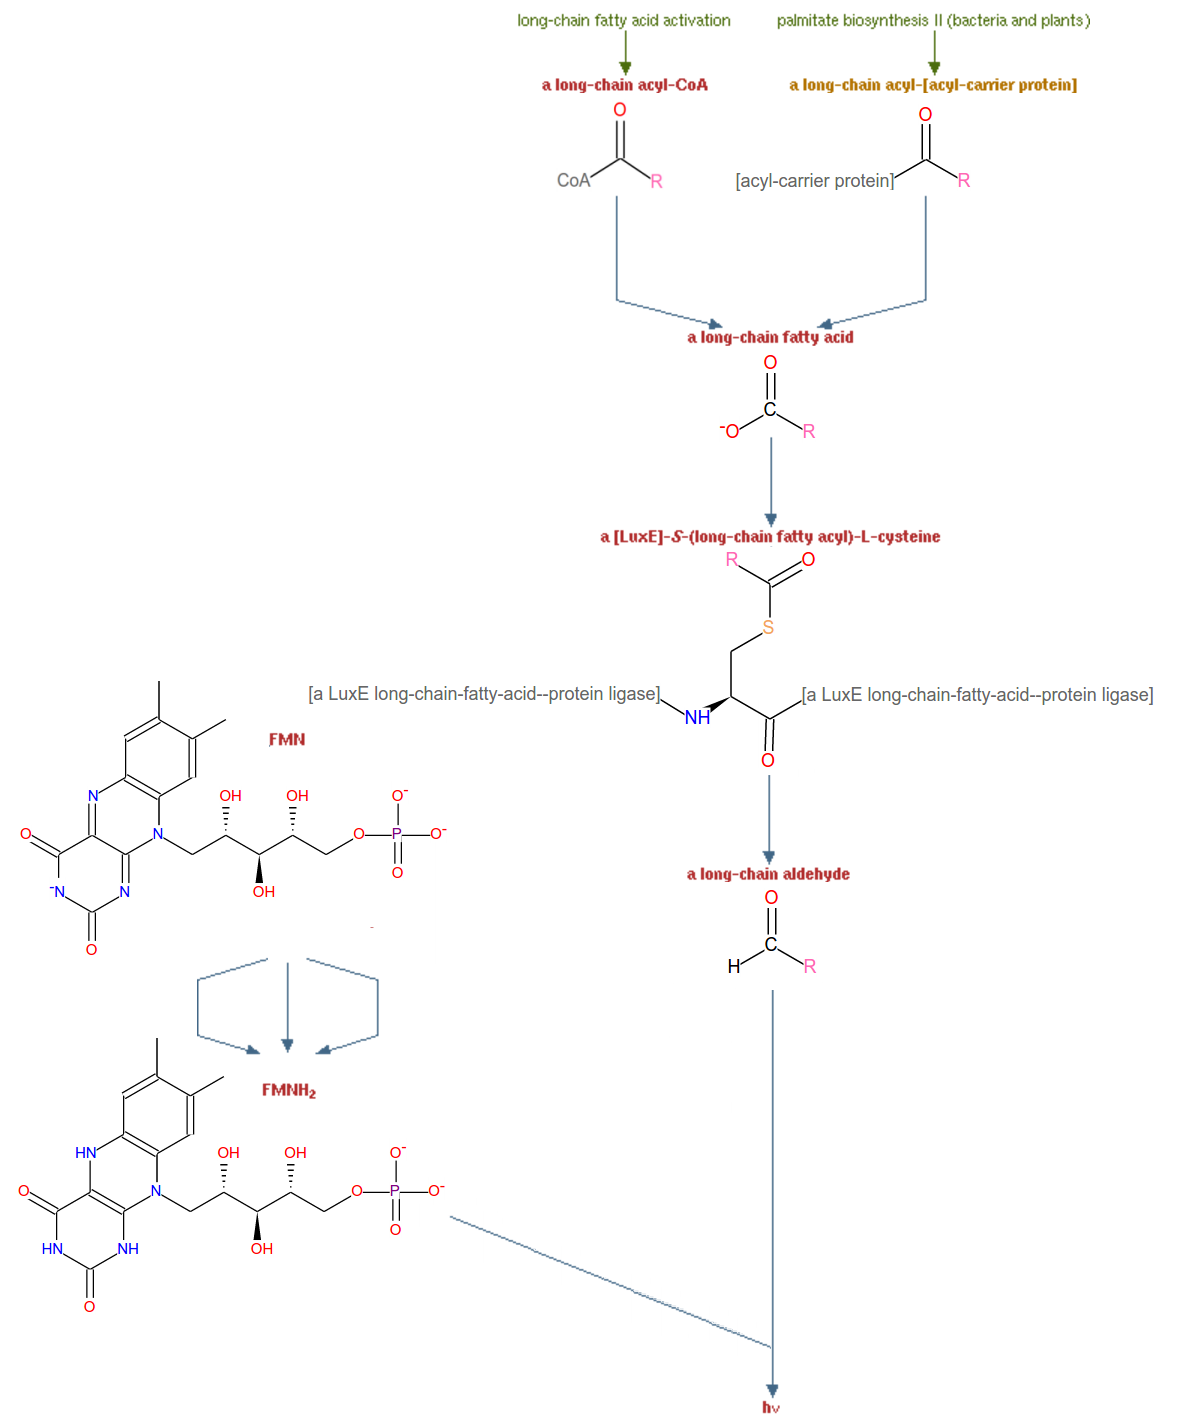
\includegraphics[width=1\textwidth]{bioLuz_id.png}
\caption{Representação modificada da Figura \ref{fig:bioLuz} com maior nível de detalhes apresentada pelo MetaCyc.}
\label{bioLuz_id}
\end{figure}

% ____________________________________________________________________
% ____________________________________________________________________
% ____________________________________________________________________


\subsection{2Path}

\indent Conteúdo estará disponível quando site estiver pronto. \\

%\cite{lacroixCTS08}

% ____________________________________________________________________
% _____________FIGURAS MAIORES NO FIM DO CAPITULO_____________________
% ____________________________________________________________________
